\chapter{Effects of soil microbes on plant competition: a perspective from modern coexistence theory: Appendices S1 -- S4}
%\chaptermark{Positive frequency-dependence}
%\renewcommand{\sectionmark}[1]{}
\fancyhead[LE, RO]{\thepage}
\fancyhead[RE]{APPENDIX C}
\fancyhead[LO]{SOIL MICROBES AND PLANT COEXISTENCE}
\fancyfoot{}
\renewcommand{\headrulewidth}{0pt}
\setlength{\parindent}{1cm}


\begin{comment}
\documentclass[hidelinks,12pt]{article}
\usepackage{graphicx,bm, booktabs,lineno,array}
\usepackage[fleqn]{amsmath}
\setlength{\mathindent}{0pt}
\usepackage[super,comma,numbers, compress]{natbib}
\usepackage[a4paper]{geometry}
\usepackage[parfill]{parskip}
\usepackage[usenames,dvipsnames]{color}
\usepackage[font=footnotesize,labelfont=bf,margin=1cm, labelsep = none]{caption} 
\usepackage{setspace}
\usepackage{gensymb}
\usepackage{color} 
\usepackage{sidecap}
\usepackage{epigraph}
\usepackage{float}
\usepackage{soul,xcolor}
\setstcolor{red}
\setlength\epigraphwidth{12cm}
\setlength\epigraphrule{0pt}
\usepackage{etoolbox}
\usepackage{tcolorbox}
\tcbuselibrary{breakable}
\usepackage[bottom, symbol]{footmisc}
\usepackage{authblk}
\usepackage{hyperref}
\usepackage[color=cyan]{todonotes}
\pdfminorversion=3
\doublespacing

\renewcommand{\epigraphflush}{center}
\renewcommand{\sourceflush}{flushleft}
\newcommand{\plus}{\raisebox{.4\height}{\scalebox{.6}{+}}}
\newcommand{\minus}{\raisebox{.4\height}{\scalebox{.8}{-}}}
\renewcommand{\thefootnote}{\fnsymbol{footnote}}
\newcommand*\samethanks[1][\value{footnote}]{\footnotemark[#1]}
\newcommand\blfootnote[1]{%
\begingroup
\renewcommand\thefootnote{}\footnote{#1}%
\addtocounter{footnote}{-1}%
\endgroup
}
\end{comment}



\begin{comment}
\begin{document}

\doublespacing
\title{Effects of soil microbes on plant competition: \\ a perspective from modern coexistence theory}
\author[* 1]{Po-Ju Ke}
\author[* 1, 2]{Joe Wan}
\affil[1]{Department of Biology, Stanford University, Stanford, California 94305-5020, USA}
\affil[2]{Institute of Integrative Biology, Department of Environmental Systems Science, ETH Z\"{u}rich, 8092 Z\"{u}rich, Switzerland}
\date{}
\maketitle
\blfootnote{* Both authors contributed equally}
\blfootnote{Correspondence author: Department of Biology, Stanford University, Stanford, California 94305-5020, USA. Phone: +1 650-721-1711. Email: pojuke@stanford.edu, jwan@student.ethz.ch}

\onehalfspacing
\noindent \textbf{Type of article:} Concepts and Synthesis\\
\noindent \textbf{Running head:} Soil microbes and plant coexistence\\
% \noindent \textbf{Keywords:} fitness difference, mutualism, niche difference, pathogens, plant--soil feedback\\
% \begin{myindentpar}{1cm}
	\textbf{Words in Abstract:} 233\\
	\textbf{Words in main text:} 7658\\
	% \textbf{Words in text boxes:} 241\\
	\textbf{Number of references:} 65\\
	\textbf{Number of figures:} 5\\
	\textbf{Number of tables:} 1\\
	\textbf{Number of text boxes:} 2\\
% \end{myindentpar}

% \noindent \textbf{Authorship statement:} PJK conceived the study; PJK and JW performed the analysis and wrote the manuscript.\\

% \noindent \textbf{Data accessibility statement:} No original data appear in this manuscript. Should the manuscript be accepted, all computer scripts supporting the results will be archived in an appropriate public repository such as Github, with the DOI included at the end of the article.\\

\doublespacing
\linenumbers
\end{comment}



\section{Appendix S1 -- Deriving the general plant--soil microbe interaction model from other candidate models}
To illustrate how modern coexistence theory can be applied to study plant-soil microbe interactions, in the main text we used \citet{Eppinga2006} as an example model. While we demonstrated how this model can be converted to a phenomenological Lotka-Volterra form, it is not the only modeling possibility -- under some circumstances other models may be more suitable. Here, we briefly show how our approach can be applied to two other potential models, which cover a wide range of dynamics between plants and their associated soil microbial community.
\par


\subsubsection*{Resource uptake as the process governing plant--plant competition}
We consider a model that explicitly captures resource competition as the mechanism behind plant--plant competition. The full three-trophic level model closely follows the model in \citet{Chesson2008b}. The density of soil resources are represented by $R_{l}$ ($l=1$ or $2$), whereas the density of plants and soil microbes are represented by $N_{i}$ and $S_{i}$ ($i=A$ or $B$), respectively. The dynamics of the three-trophic level model is captured by the following dynamic system:

\begin{equation}
%\frac{dR_{i}}{dt} = r_{i}^{R} R_{i} \left ( 1 - \frac{R_{i} }{K_{i}^{R}} \right ) - a_{iA}R_{i}N_{A}  - a_{iB}R_{i}N_{B}
\frac{dR_{l}}{dt} = r_{l}^{R} R_{l} \left ( 1 - \frac{R_{l} }{K_{l}^{R}} \right ) - a_{lA}R_{l}N_{A}  - a_{lB}R_{l}N_{B}
\tag{S4.1}\label{eq:Resource_RCmodel}
\end{equation}
\begin{equation}
%\frac{dN_{i}}{dt} = e_{Ai}a_{Ai}R_{A}N_{i}  + e_{Bi}a_{Bi}R_{B}N_{i} + \left( \sigma_{iA}S_{A}+\sigma_{iB}S_{B} \right)N_{i} - d_{i}N_{i}
\frac{dN_{i}}{dt} = e_{1i}a_{1i}R_{1}N_{i}  + e_{2i}a_{2i}R_{2}N_{i} + \left( \sigma_{iA}S_{A}+\sigma_{iB}S_{B} \right)N_{i} - d_{i}N_{i}
\tag{S4.2}\label{eq:Plant_RCmodel}
\end{equation}
\begin{equation}
\frac{dS_{i}}{dt } = g_{i}S_{i}\left ( 1-\frac{S_{i}}{k_{i}}\right ) .
\tag{S4.3}\label{eq:Soil_RCmodel}
\end{equation}

\noindent Here, resources follow logistic growth, with intrinsic growth rate and carrying capacity $r_{l}^{R}$ and $K_{l}^{R}$, respectively. The superscript $R$ indicates that these parameters are associated with resource dynamics. Plants compete with each other via consuming, and thus lowering the amount of available, resources: $R_{l}$ is consumed by plant species $N_{A}$ and $N_{B}$ with consumption rates $a_{lA}$ and $a_{lB}$, respectively. The two resources $R_{1}$ and $R_{2}$ are assumed to be substitutable, and contribute to plant population size $N_{i}$ after being assimilated, with conversion efficiency, $e_{1i}$ and $e_{2i}$, respectively. Plants die with density-independent morality rate, $d_{i}$. Finally, soil dynamics are assumed to follow the same dynamics as Eqns.~\ref{eq:SoilA} and \ref{eq:SoilB} in the main text. Under the assumption of logistically growing resources, this model can also be simplified to a Lotka-Volterra form after applying separation of timescales (i.e., assuming both resources and soil microbes are the fast variable).
In particular, the quasi-equilibrium for resources are $\hat{R_{l}}= K_{l}^{R} - \frac{K_{l}^{R}}{r_{l}^{R}} \left ( a_{lA}N_{A}+a_{lB}N_{B} \right )$, whereas that for soil microbes are $\hat{S_{i}}= \phi_{i} \times N_{i}$. Substituting these expressions into Eqn.~\ref{eq:Plant_RCmodel}:

\makeatletter
\def\tagform@#1{\maketag@@@{\normalsize(#1)\@@italiccorr}}
\makeatother
\footnotesize
\begin{equation}
\begin{split}
\frac{dN_{A}}{dt}\frac{1}{N_{A}}& = \left ( e_{1A}a_{1A}K_{1}^{R} + e_{2A}a_{2A}K_{2}^{R} - d_{A} \right ) \times \\
& \quad \left [ 1 +
\left ( -\frac{ K_{1}^{R}}{r_{1}^{R}}e_{1A}a_{1A}^{2} - \frac{K_{2}^{R}}{r_{2}^{R}}e_{2A}a_{2A}^{2} + \sigma_{AA}\phi_{A} \right )\frac{N_{A}}{r_{A}}
+ \left ( -\frac{ K_{1}^{R}}{r_{1}^{R}}e_{1A}a_{1A}a_{1B} - \frac{K_{2}^{R}}{r_{2}^{R}}e_{2A}a_{2A}a_{2B} + \sigma_{AB}\phi_{B} \right )\frac{N_{B}}{r_{A}} \right ]
\end{split}
\tag{S4.4}\label{eq:LVA_RCmodel}
\end{equation}
\begin{equation}
\begin{split}
\frac{dN_{B}}{dt}\frac{1}{N_{B}}& = \left ( e_{1B}a_{1B}K_{1}^{R} + e_{2B}a_{2B}K_{2}^{R} - d_{B} \right ) \times \\
& \quad \left [ 1 +
\left ( -\frac{ K_{1}^{R}}{r_{1}^{R}}e_{1B}a_{1B}a_{1A} - \frac{K_{2}^{R}}{r_{2}^{R}}e_{2B}a_{2B}a_{2A} + \sigma_{BA}\phi_{A} \right )\frac{N_{A}}{r_{B}}
+ \left ( -\frac{ K_{1}^{R}}{r_{1}^{R}}e_{1B}a_{1B}^{2} - \frac{K_{2}^{R}}{r_{2}^{R}}e_{2B}a_{2B}^{2} + \sigma_{BB}\phi_{B} \right )\frac{N_{B}}{r_{B}} \right ]
\end{split}
\tag{S4.5}\label{eq:LVB_RCmodel}
\end{equation}
\normalsize

\noindent where $r_{i} = e_{1i}a_{1i}K_{1}^{R} + e_{2i}a_{2i}K_{2}^{R} - d_{i}$. The interaction coefficient among competing plants, $\alpha_{ij}$, can be written as:

\begin{equation}
\alpha_{ij} =
\left ( \frac{-\frac{ K_{1}^{R}}{r_{1}^{R}}e_{1i}a_{1i}a_{1j} - \frac{K_{2}^{R}}{r_{2}^{R}}e_{2i}a_{2i}a_{2j}}
{e_{1i}a_{1i}K_{1}^{R} + e_{2i}a_{2i}K_{2}^{R} - d_{i}}\right )
+ \left ( \frac{\sigma_{ij}\phi_{j}}
{e_{1i}a_{1i}K_{1}^{R} + e_{2i}a_{2i}K_{2}^{R} - d_{i}}\right ).
\tag{S4.6}\label{eq:alpha_RCmodel}
\end{equation}

\noindent The above expression takes the same form as Eqn.~\ref{eq:alpha} in the main text, and thus can be thought as a mechanistic decomposition of Eqn.~\ref{eq:alpha}. In particular, the term enclosed in the first parenthesis represents plant--plant competition whereas the second parenthesis represents plant--soil microbe interactions. Note that since we are modeling plant--plant competition via resource uptake, the first term in Eqn.~\ref{eq:alpha_RCmodel} would always be negative (i.e., negative $c_{ij}$ in the main text).
With this expression of $\alpha_{ij}$, one can then calculate the niche overlap and fitness ratio between $N_{A}$ and $N_{B}$ using the equations provided in \citet{Chesson1990, Chesson2008b}.
\par


\subsubsection*{Soil microbes are conditioned by both plant species}
In our modified \citet{Eppinga2006} model, soil microbial community $S_{i}$ exhibits strong host specificity and is only conditioned by plant $N_{i}$. In some systems, soil microbes might be more generalists and are conditioned by both plant species (i.e., $N_{i}$ conditions not only $S_{i}$ but also $S_{j}$). In this model, we assume a host-specificity conditioning ratio, $h_{i}$, for each plant species: $N_{i}$ allocates proportion $h_{i}$ of its conditioning ability, $\phi_{i}$ to soil microbial community $S_{i}$ and proportion $\left(1-h_{i}\right)$ to $S_{j}$. The dynamics of this dynamic sysem can be represented as follows:

\begin{equation}
%\frac{dN_{i}}{dt} = r_{i}N_{i} \left( 1 + \frac{c_{ii}N_{i}+c_{ij}N_{j}}{K_{i}} \right) + \left( \sigma_{ii}'S_{i}+\sigma_{ij}'S_{j} \right)N_{i}
\frac{dN_{i}}{dt} = r_{i}N_{i} \left( 1 + c_{ii}N_{i}+c_{ij}N_{j} + \sigma_{ii}'S_{i}+\sigma_{ij}'S_{j} \right)N_{i}
\tag{S4.7}\label{eq:Plant_Cocondition}
\end{equation}
\begin{equation}
\frac{dS_{i}}{dt } = g_{i}S_{i}\left ( 1-\frac{S_{i}}{k_{i}}\right ) .
\tag{S4.8}\label{eq:Soil_Cocondition}
\end{equation}

\noindent In this model, both $N_{i}$ and $N_{j}$ condition soil microbial community $S_{i}$, and the microbial community affects plant performance with interaction coefficient $\sigma_{ij}'$. The carrying capacity of soil microbes, $k_{i}$, is:

\begin{equation}
%k_{i}=h_{i}\frac{N_{i}}{K_{i}}\phi_{i} + \left ( 1-h_{j} \right )\frac{N_{j}}{K_{j}}\phi_{j}.
k_{i} = h_{i}\phi_{i}N_{i} + \left ( 1-h_{j} \right )\phi_{j}N_{j} .
\tag{S4.9}\label{eq:SoilCarrying_Cocondition}
\end{equation}

\noindent By applying the separation of timescales with the assumption that soil microbes are the fast variable compared to plants, we obtain the following Lotka-Volterra:

\makeatletter
\def\tagform@#1{\maketag@@@{\normalsize(#1)\@@italiccorr}}
\makeatother
\footnotesize
\begin{equation}
\frac{dN_{A}}{dt}\frac{1}{N_{A}} = r_{A} \left [ 1 +
\left ( c_{AA} + \sigma_{AA}'h_{A}\phi_{A} + \sigma_{AB}'\left ( 1-h_{A} \right )\phi_{A} \right )N_{A} + \left ( c_{AB} + \sigma_{AB}'h_{B}\phi_{B} + \sigma_{AA}'\left ( 1-h_{B} \right ) \phi_{B} \right )N_{B} \right ]
\tag{S4.10}\label{eq:LVA_Cocondition}
\end{equation}
\begin{equation}
\frac{dN_{B}}{dt}\frac{1}{N_{B}} = r_{B} \left [ 1 +
\left ( c_{BA} + \sigma_{BA}'h_{A}\phi_{A} + \sigma_{BB}'\left ( 1-h_{A} \right ) \phi_{A} \right )N_{A} + \left ( c_{BB} + \sigma_{BB}'h_{B}\phi_{B} + \sigma_{BA}'\left ( 1-h_{B} \right )\phi_{B} \right )N_{B} \right ]
\tag{S4.11}\label{eq:LVB_Cocondition}
\end{equation}
\normalsize

\noindent With the above equation, one then derive the intra- and inter-specific plant--plant interaction coefficients, $\alpha_{ii}$ and $\alpha_{ij}$, as follows:

\begin{equation}
\alpha_{ii} = c_{ii} + \left [ \sigma_{ii}'h_{i} + \sigma_{ij}'\left ( 1-h_{i} \right ) \right ]\phi_{i}
\tag{S4.12}\label{eq:alpha_Cocondition_con}
\end{equation}
\begin{equation}
\alpha_{ij} = c_{ij} + \left [ \sigma_{ij}'h_{j} + \sigma_{ii}'\left ( 1-h_{j} \right ) \right ]\phi_{j} .
\tag{S4.13}\label{eq:alpha_Cocondition_heter}
\end{equation}

\noindent The above expression takes the same form as Eqn.~\ref{eq:alpha} in the main text, with $\sigma_{ij}$ being partitioned into effects coming from two different soil microbial communities (i.e., the $\sigma_{ij}'$ and $\sigma_{ii}'$ terms enclosed in the bracket).
As one can observe, this model reduces to our modified \citet{Eppinga2006} model when plants only condition their associated soil microbes (i.e., $h_{i}=h_{j}=1$). An alternative way to interpret this new expression is that our original $\sigma_{ij}$ (Eqn.~\ref{eq:alpha}) is a phenomenological summary of its separated components. Again, with this expression of $\alpha_{ij}$, one can then calculate the niche overlap and fitness ratio between $N_{A}$ and $N_{B}$.
\par



\section{Appendix S2 -- Separating stabilizing and equalizing components}
To calculate the components of modern coexistence theory, we applied separation of timescales to reduce the dimensions of our model (Eqns. \ref{eq:SoilA}-\ref{eq:Nb}) to a Lotka--Volterra, an approach that was also used in many classic studies \citep{MacArthur1970, Chesson1990}. In particular, we assumed that the dynamics of soil microbes are sufficiently fast (the fast variable) compared to that of the plants (the slow variable) and all dynamics occur near the equilibrium. These assumptions allowed us to calculate the quasi-equilibrium of the two soil communities, $\hat{S_{i}}$, by setting Eqns.~\ref{eq:SoilA} and \ref{eq:SoilB} in the main text as zero and assuming the slow variables are unchanging:

\begin{equation}
%\hat{S_{i}}= k_{i}= \frac{N_{i}}{K_{i}}\times \phi_{i}
\hat{S_{i}}= k_{i}= N_{i} \times \phi_{i}
\tag{S4.14} \label{eq:QuasiSoil}
\end{equation}

\noindent where $i = A$ or $B$. To understand the dynamics of the slow variable, we substituted this quasi-equilibrium into Eqns.~\ref{eq:Na} and \ref{eq:Nb} by assuming the soil communities always remain near their quasi-equilibrium:

\begin{equation}
\frac{dN_{A}}{dt } = r_{A}N_{A}\left [1 + \left(c_{AA}+\sigma_{AA}\phi_{A}\right)N_{A} + \left(c_{AB}+\sigma_{AB}\phi_{B}\right)N_{B}\right ]
\tag{S4.15}\label{eq:NaLV}
\end{equation}
\begin{equation}
\frac{dN_{B}}{dt } = r_{B}N_{B}\left [1 + \left(c_{BA}+\sigma_{BA}\phi_{A}\right)N_{A} + \left(c_{BB}+\sigma_{BB}\phi_{B}\right)N_{B}\right ] .
\tag{S4.16}\label{eq:NbLV}
\end{equation}

\noindent The resulting simplified model is a two species Lotka--Volterra model, with species' per capita growth rate as a linear function of intra- and inter-specific densities.
The interaction coefficients, $\alpha_{ij}$, shown below in equation \ref{eq:S_alpha}, consist of both plant--plant competition that are not related to soil microbes, $c_{ij}$, and soil microbial effects, summarized as $\sigma_{ij}\phi_{j}$.
We assumed plant--plant interactions are competitive ($c_{ij} < 0$) whereas plant--soil microbe interactions can be either detrimental ($\sigma_{ij} < 0$) or beneficial ($\sigma_{ij} > 0$). Our model simplifies to the classic Lotka--Volterra competition model when $\sigma_{ij}$ or $\phi_{i} = 0$:

\begin{equation}
\alpha_{ij} = c_{ij} + \sigma_{ij}\phi_{j} .
\tag{S4.17}\label{eq:S_alpha}
\end{equation}

\noindent After transforming the model into a Lotka--Volterra form, we can now quantify niche overlap and fitness ratio among the two plants \citep{Chesson1990, Chesson2008b, Chesson2013ecosys}. Note that the following analytical definition of these terms were derived specifically for a two-species Lotka--Volterra framework. Thus, it ignores other coexistence mechanisms that rely on temporal fluctuation and spatial variation (but see \cite{Chesson2003, Barabas2018} for a more generalizable definition of these components). With this formalization, stabilizing mechanisms represent processes that decrease niche overlap, $\rho$ (or increases niche difference, $1-\rho$). Here, $\rho$ is defined as a symmetric measure of the ratio of inter- to intra-specific density dependence based on Lotka--Volterra coefficients, i.e., $\rho = \sqrt{\frac{\alpha_{BA}\alpha_{AB}}{\alpha_{AA}\alpha_{BB}}}$. Accordingly, we derived the niche overlap between $N_{A}$ and $N_{B}$ as:

\begin{equation}
\rho = \sqrt{\frac{\left ( c_{BA} + \sigma_{BA}\phi_{A} \right )
						   \left ( c_{AB} + \sigma_{AB}\phi_{B} \right )}
						  {\left ( c_{AA} + \sigma_{AA}\phi_{A} \right )
						   \left ( c_{BB} + \sigma_{BB}\phi_{B} \right )}} .
\tag{S4.18}\label{eq:S_ND}
\end{equation}

\noindent Equalizing mechanisms, on the other hand, represent processes that reduce the fitness ratio between species, which is defined as $\frac{f_{B}}{f_{A}} = \sqrt{\frac{\alpha_{AA}\alpha_{AB}}{\alpha_{BB}\alpha_{BA}}}$. According, we derived this term for our model as:

\begin{equation}
\frac{f_{B}}{f_{A}} = \sqrt{\frac{\left ( c_{AA} + \sigma_{AA}\phi_{A} \right )
											    \left ( c_{AB} + \sigma_{AB}\phi_{B} \right )}
											   {\left ( c_{BB} + \sigma_{BB}\phi_{B} \right )
												\left ( c_{BA} + \sigma_{BA}\phi_{A} \right )}} .
\tag{S4.19}\label{eq:S_FR}
\end{equation}
\par



\section{Appendix S3 -- Invasion analysis for the plant--soil microbe interaction model}
Here, we perform invasion analysis and demonstrate how it aids understanding for our results. This is done by assuming that one of the two species (the invader) is at low density while the other (the resident) is at its mono-dominance equilibrium, such that the invader is affected by the resident but itself has no effects on its surroundings. Under such scenario, the per capita growth rate of the resident is zero and that for the invader is called its invasion growth rate (IGR). If both species, when as the invader, have positive invasion growth rates, they can stably coexist as both are able to recover from low density. To see how this works, let us first consider a two-species Lotka--Volterra competition model:

\begin{equation}
\frac{dN_{A}}{dt} = r_{A}N_{A}\left ( 1-\alpha_{AA}N_{A}-\alpha_{AB}N_{B} \right )
\tag{S4.20}\label{eq:S_LVA}
\end{equation}
\begin{equation}
\frac{dN_{B}}{dt} = r_{B}N_{B}\left ( 1-\alpha_{BA}N_{A}-\alpha_{BB}N_{B} \right ) .
\tag{S4.21}\label{eq:S_LVB}
\end{equation}

\noindent First, assume $N_{A}$ is at invader state and $N_{B}$ is at its mono-dominance equilibrium, $\frac{1}{\alpha_{BB}}$, which is obtained by setting equation \ref{eq:S_LVB} to zero under $N_{A}$ equal zero. The invasion growth rate of $N_{A}$, $IGR_{A}$ is derived as:

\begin{equation}
IGR_{A} =
\left.\begin{matrix}
\frac{1}{N_{A}}\frac{dN_{A}}{dt}
\end{matrix}\right|
_{N_{A}=0, N_{B}=\frac{1}{\alpha_{BB}}} = r_{A}\left( 1 - \frac{\alpha_{AB}}{\alpha_{BB}}\right) .
\tag{S4.22}\label{eq:S_IGR_A}
\end{equation}

\noindent If $IGR_{A}$ is greater than zero, then $N_{A}$ can recover from arbitrarily low density, preventing itself from being excluded. As mentioned, it is important to observe that the sign of $IGR_{A}$ depends solely on the intra- and inter-specific interaction coefficients of $N_{B}$ ($\alpha_{BB}$ and $\alpha_{AB}$, respectively). This makes sense: $N_{A}$, as the invader, is too rare to have any impact on the surroundings and thus its growth rate is only determined by the impact from the resident species. The same process applies when $N_{B}$ is the invader and $N_{A}$ is at its mono-dominance equilibrium, $\frac{1}{\alpha_{AA}}$. Note that while this method can be generalized to $n-$species community, careful thought needs to be given when considering the coexistence of all the combinations of remaining $n-1$ species \citep{Barabas2018}. For two species simple Lotka--Volterra there is no problem since if one species goes extinct, the other one will always persist.
\par


Now, we can perform invasion analysis for our simplified plant--soil interaction model (Eqns.~\ref{eq:NaLV} and \ref{eq:NbLV}), which takes the form of a simple two-species Lotka--Volterra model as shown in Eqns.~\ref{eq:S_LVA} and \ref{eq:S_LVB}. The invasion growth rate will thus take the same form as Eqn \ref{eq:S_IGR_A}, with $\alpha_{ij}$ following \ref{eq:S_alpha}:

\begin{equation}
IGR_{A} =
r_{A}\left [ 1 - \left ( \frac{c_{AB}+\sigma_{AB}\phi_{B}} {c_{BB}+\sigma_{BB}\phi_{B}} \right ) \right ]
\tag{S4.23}\label{eq:IGR_A}
\end{equation}
\begin{equation}
IGR_{B} =
r_{B}\left [ 1 - \left ( \frac{c_{BA}+\sigma_{BA}\phi_{A}} {c_{AA}+\sigma_{AA}\phi_{A}} \right ) \right ] .
\tag{S4.24}\label{eq:IGR_B}
\end{equation}
\par



\clearpage
\section{Appendix S4 -- Supplementary Tables and Figures}
\begin{table}[h]
	\centerfloat
	\caption[Default parameter values for each plant--soil microbe interaction scenario.]
	{Default parameter values for each plant--soil microbe interaction scenario (see main text for the detailed simulation process and the range of parameter variation for plant-mediated competition, $c_{ij}$).}
	\label{table:Parameters}
	\begin{tabular}{lcccc}
		\toprule \textbf{Parameter} & \textbf{Janzen-Connell} & \textbf{enemy release} & \textbf{mutual facilitation} & \textbf{soil conditioning} \tabularnewline
		\midrule
		\midrule
		$\phi_{A}$    &  1.6          &  0.5      &  0.15       &  0.025 \tabularnewline
		$\phi_{B}$    &  2.0          &  0.5      &  0.20       &  0.025 -- 2.5 \tabularnewline
		$\sigma_{AA}$ & -0.32 -- -6.0 & -0.5      &  0.5        &  0.50 \tabularnewline
		$\sigma_{AB}$ & -0.4          & -0.5      &  0.0 -- 2.0 &  0.25 \tabularnewline
		$\sigma_{BB}$ & -0.32 -- -6.0 & -2.0 -- 0 &  0.5        &  0.20 \tabularnewline
		$\sigma_{BA}$ & -0.5          & -2.0 -- 0 &  0.0 -- 2.0 &  0.10 \tabularnewline
		$c_{AA}$      & -1.0          & -1.5      & -1.0        & -1.0 \tabularnewline
		$c_{AB}$      & -1.0          & -1.0      & -1.0        & -1.0 \tabularnewline
		$c_{BB}$      & -0.8          & -1.5      & -1.0        & -0.9 \tabularnewline
		$c_{BA}$      & -0.8          & -1.0      & -1.0        & -0.9 \tabularnewline
		\bottomrule
	\end{tabular}%
\end{table}
\bigskip\bigskip\bigskip\bigskip
\bigskip\bigskip\bigskip\bigskip



\clearpage
\begin{figure}[htbp]
	\centering
	\makebox[\textwidth][c]{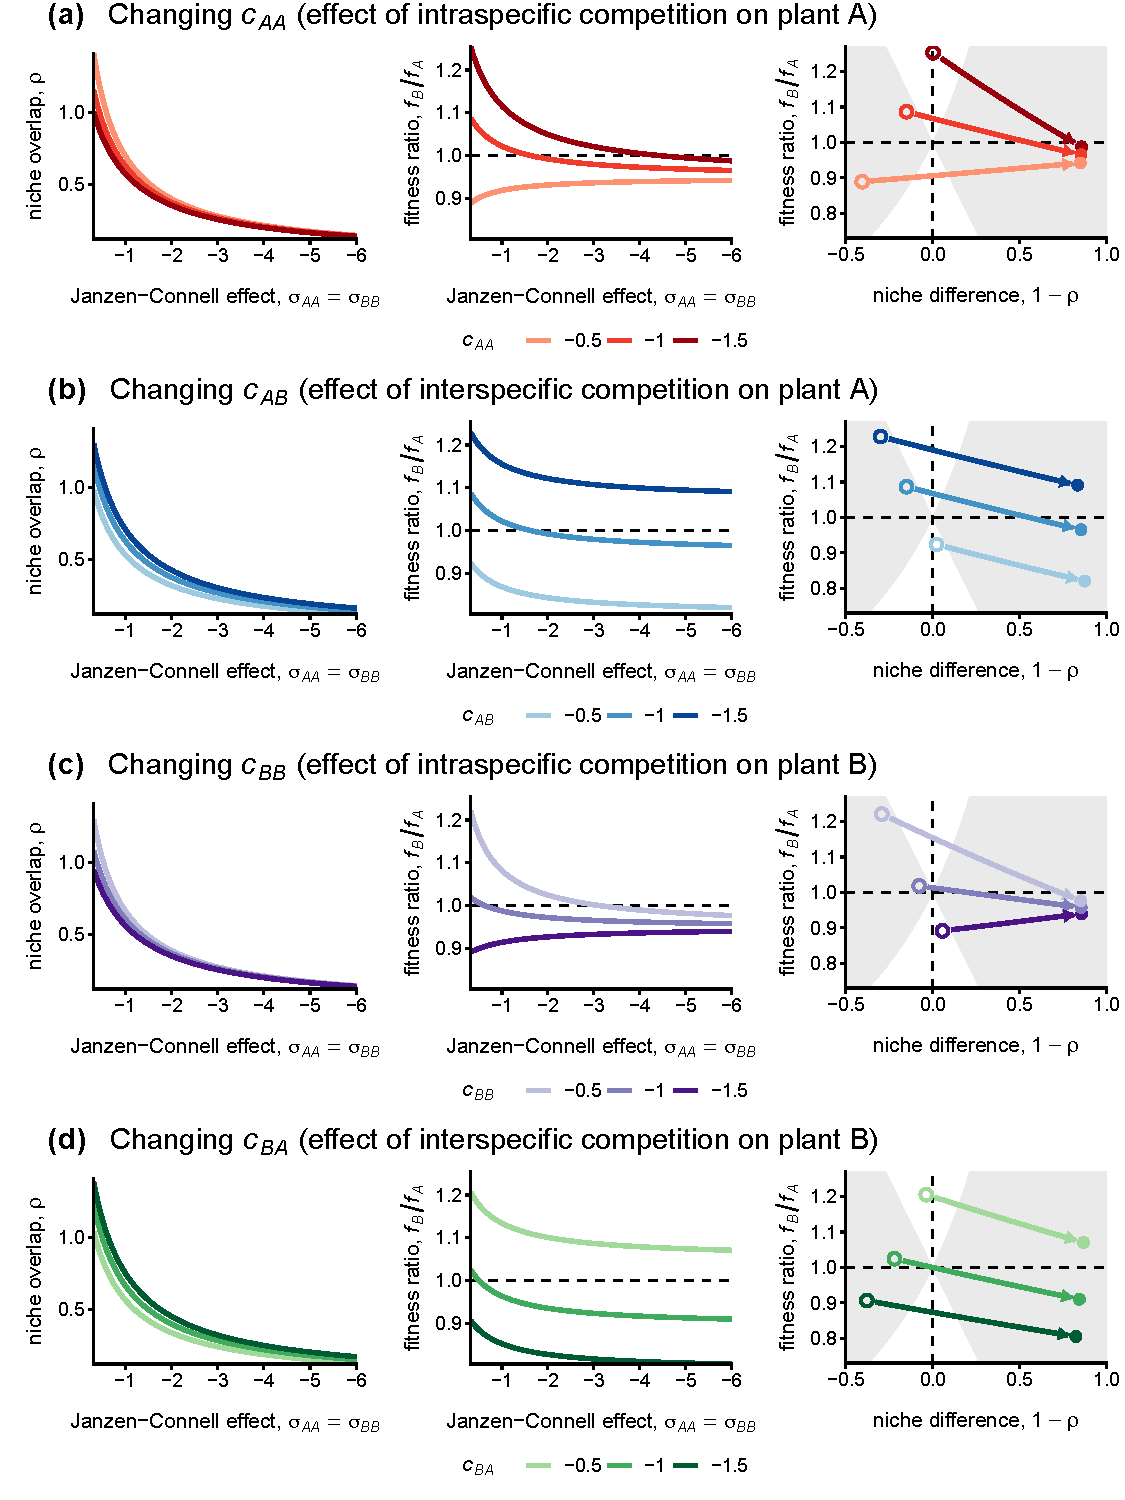
\includegraphics[width=12cm]{Chapter4/Translated_Janzen_Connell_full.pdf}}
	\caption[The effects of varying plant--soil microbe interactions ($\sigma_{AA}$ and $\sigma_{BB}$) and plant--plant competition on competitive outcomes for the Janzen--Connell scenario.]
		{The effects of varying plant--soil microbe interactions ($\sigma_{AA}$ and $\sigma_{BB}$) and plant--plant competition on competitive outcomes for the Janzen--Connell scenario.
		Each row (panel a--d) represent the effects of varying one plant--plant competition coefficient while keeping the other three constant: (a) $c_{AA}$, in red colors; (b) $c_{AB}$, in blue colors; (c) $c_{BB}$, in purple colors; (d) $c_{BA}$, in green colors. Lines with different brightness represent different plant--plant competition strength, ranging from weak (light colors) to strong (dark colors).
		The first two columns represent the effects of varying $\sigma_{AA}$ and $\sigma_{BB}$ on niche overlap ($\rho$) and fitness ratio ($f_{B}/f_{A}$), respectively. The third column visualizes the changes in the two components on the parameter space of niche difference ($1 - \rho$, x-axis) and fitness ratio ($f_{B}/f_{A}$, y-axis). Arrows represent the effects of changing plant--soil microbe interactions, from weakest (open circle) to strongest (solid circle). See also Fig.~\ref{fig:Scenario_Battleaxes} legend.} 
	\label{fig:Janzen_Connell_everything}
\end{figure}



\clearpage
\begin{figure}[htbp]
	\centering
	\makebox[\textwidth][c]{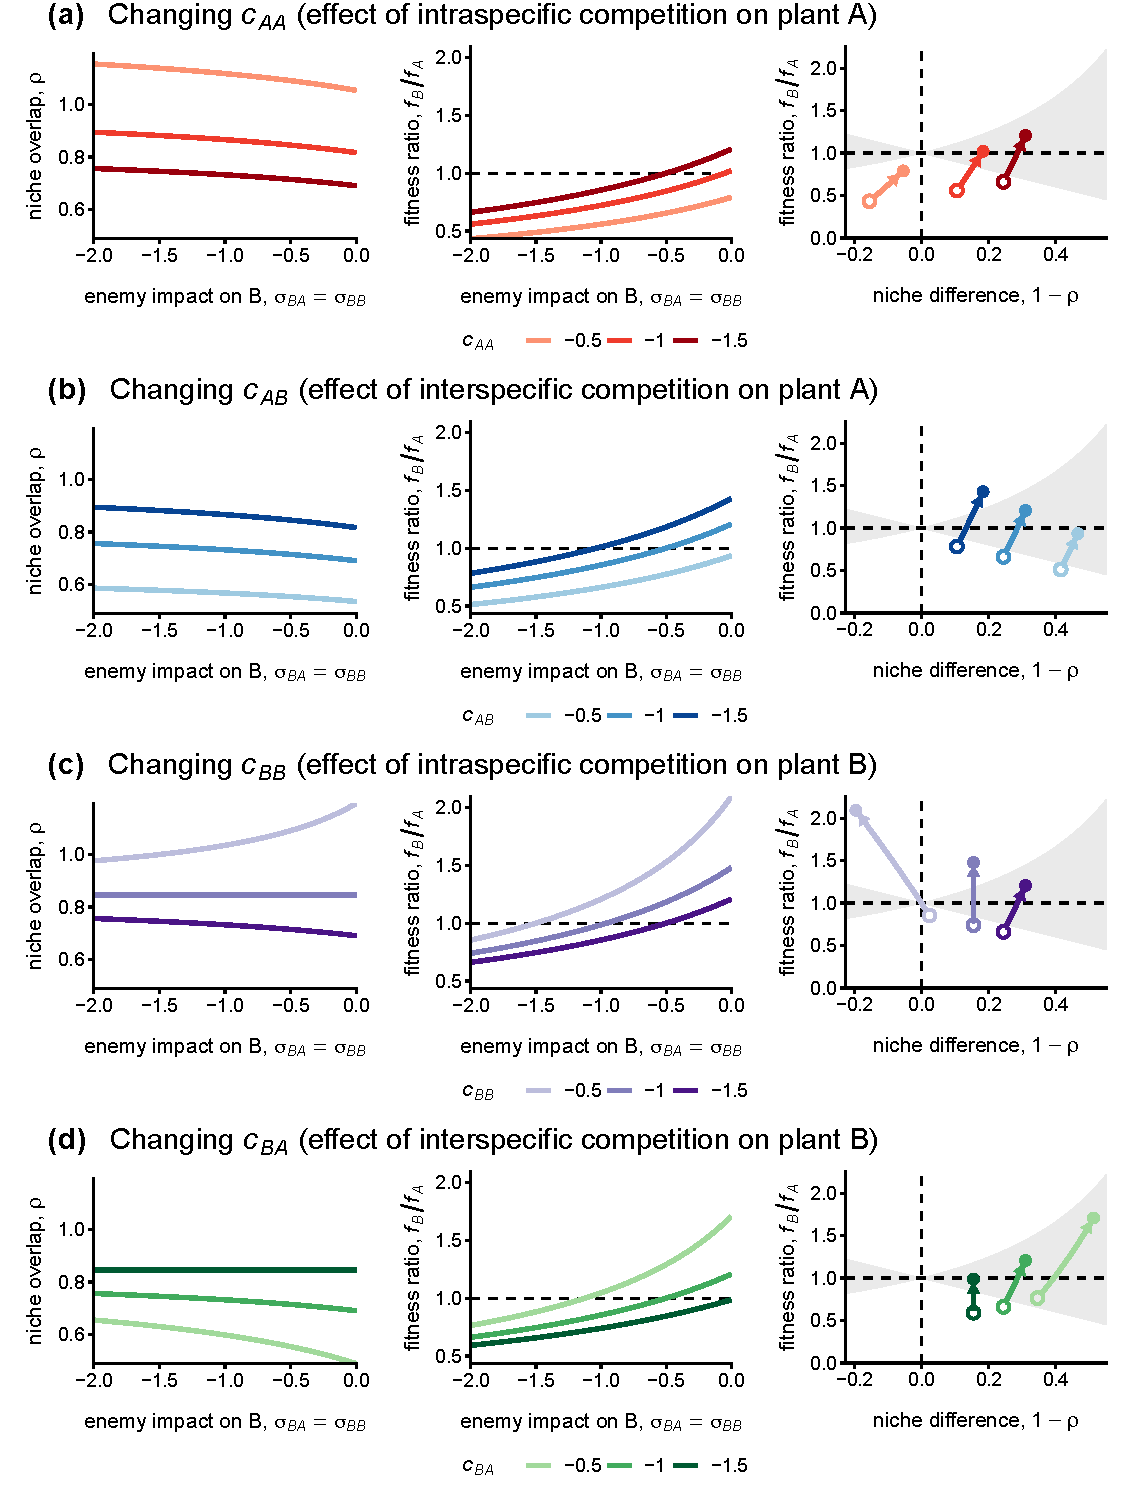
\includegraphics[width=12cm]{Chapter4/Translated_Enemy_Release_full.pdf}}
	\caption[The effects of varying plant--soil microbe interactions ($\sigma_{BA}$ and $\sigma_{BB}$) and plant--plant competition on competition outcomes for the enemy release scenario.]
		{The effects of varying plant--soil microbe interactions ($\sigma_{BA}$ and $\sigma_{BB}$) and plant--plant competition on competition outcomes for the enemy release scenario.
		Each row (panel a--d) represent the effects of varying one plant--plant competition coefficient while keeping the other three constant: (a) $c_{AA}$, in red colors; (b) $c_{AB}$, in blue colors; (c) $c_{BB}$, in purple colors; (d) $c_{BA}$, in green colors. Lines with different brightness represent different plant--plant competition strength, ranging from weak (light colors) to strong (dark colors).
		The first two columns represent the effects of varying $\sigma_{BA}$ and $\sigma_{BB}$ on niche overlap ($\rho$) and fitness ratio ($f_{B}/f_{A}$), respectively. The third column visualizes the changes in the two components on the parameter space of niche difference ($1 - \rho$, x-axis) and fitness ratio ($f_{B}/f_{A}$, y-axis). Arrows represent the effects of changing plant--soil microbe interactions, from weakest (open circle) to strongest (solid circle). See also Fig.~\ref{fig:Scenario_Battleaxes} legend.}
	\label{fig:Enemy_Release_everything}
\end{figure}



\clearpage
\begin{figure}[htbp]
	\centering
	\makebox[\textwidth][c]{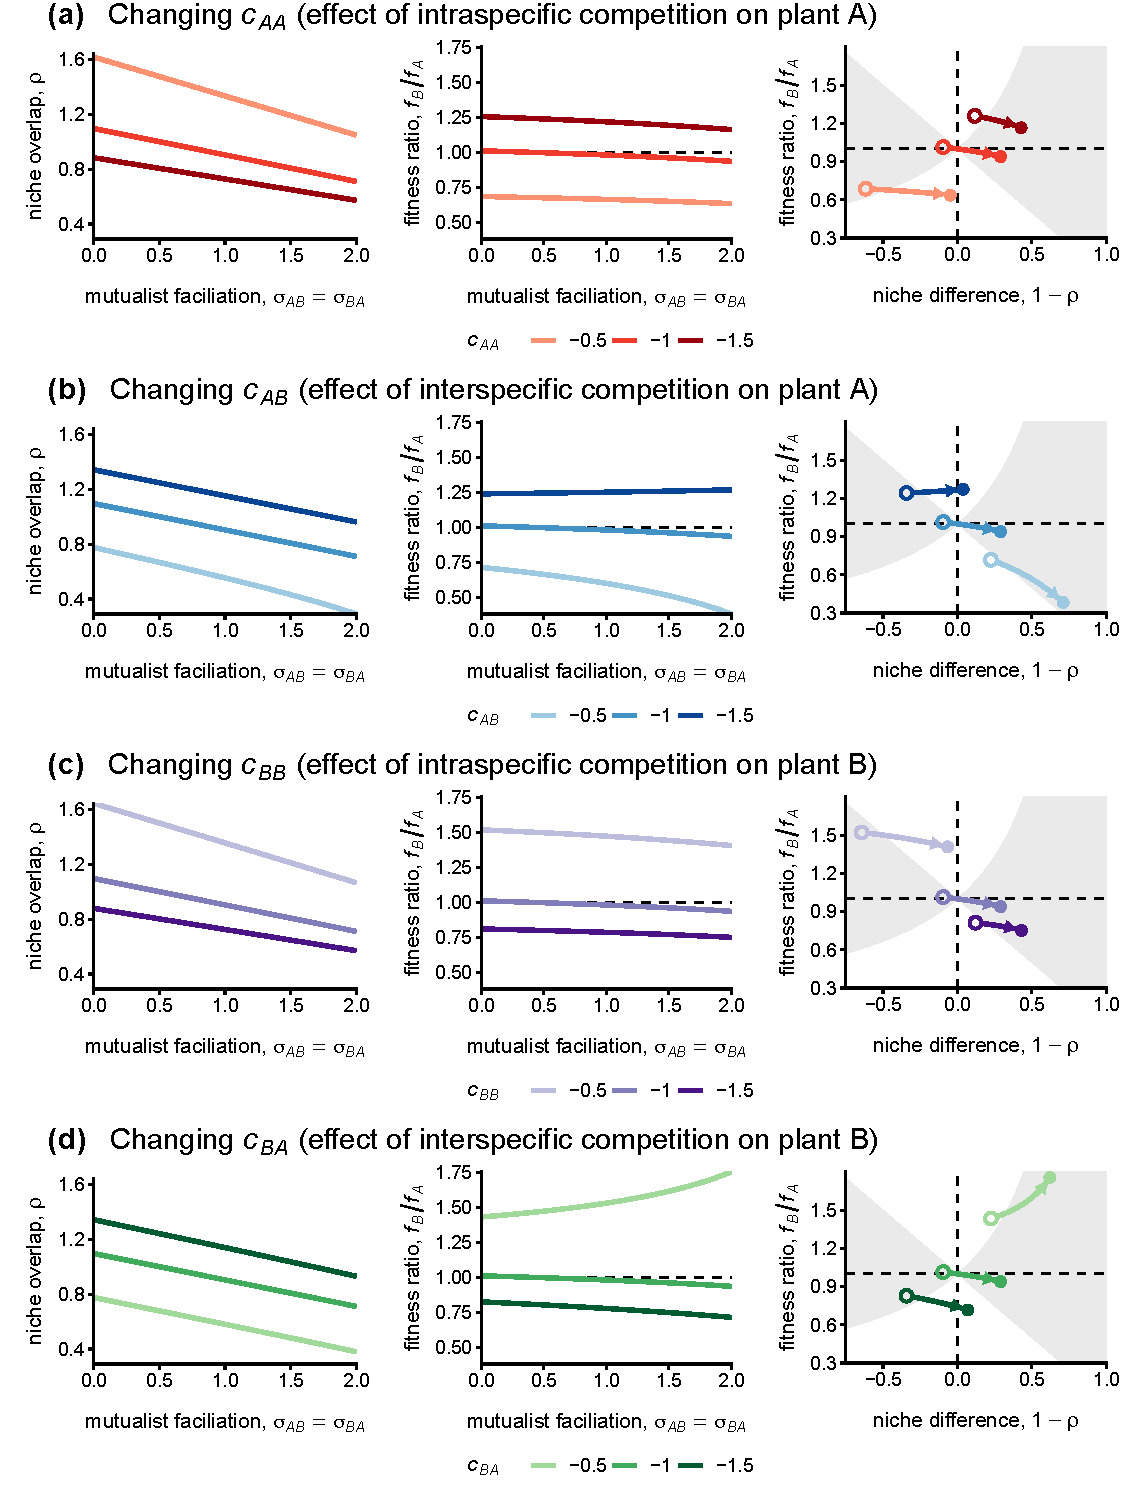
\includegraphics[width=12cm]{Chapter4/Translated_Mutual_Facilitation_full.pdf}}
	\caption[The effects of varying plant--soil microbe interactions ($\sigma_{BA}$ and $\sigma_{AB}$) and plant--plant competition on competition outcomes for the mutual facilitation scenario.]
		{The effects of varying plant--soil microbe interactions ($\sigma_{BA}$ and $\sigma_{AB}$) and plant--plant competition on competition outcomes for the mutual facilitation scenario.
		Each row (panel a--d) represent the effects of varying one plant--plant competition coefficient while keeping the other three constant: (a) $c_{AA}$, in red colors; (b) $c_{AB}$, in blue colors; (c) $c_{BB}$, in purple colors; (d) $c_{BA}$, in green colors. Lines with different brightness represent different plant--plant competition strength, ranging from weak (light colors) to strong (dark colors).
		The first two columns represent the effects of varying $\sigma_{BA}$ and $\sigma_{AB}$ on niche overlap ($\rho$) and fitness ratio ($f_{B}/f_{A}$), respectively. The third column visualizes the changes in the two components on the parameter space of niche difference ($1 - \rho$, x-axis) and fitness ratio ($f_{B}/f_{A}$, y-axis). Arrows represent the effects of changing plant--soil microbe interactions, from weakest (open circle) to strongest (solid circle). See also Fig.~\ref{fig:Scenario_Battleaxes} legend.}
	\label{fig:Mutual_Facilitation_everything}
\end{figure}



\clearpage
\begin{figure}[htbp]
	\centering
	\makebox[\textwidth][c]{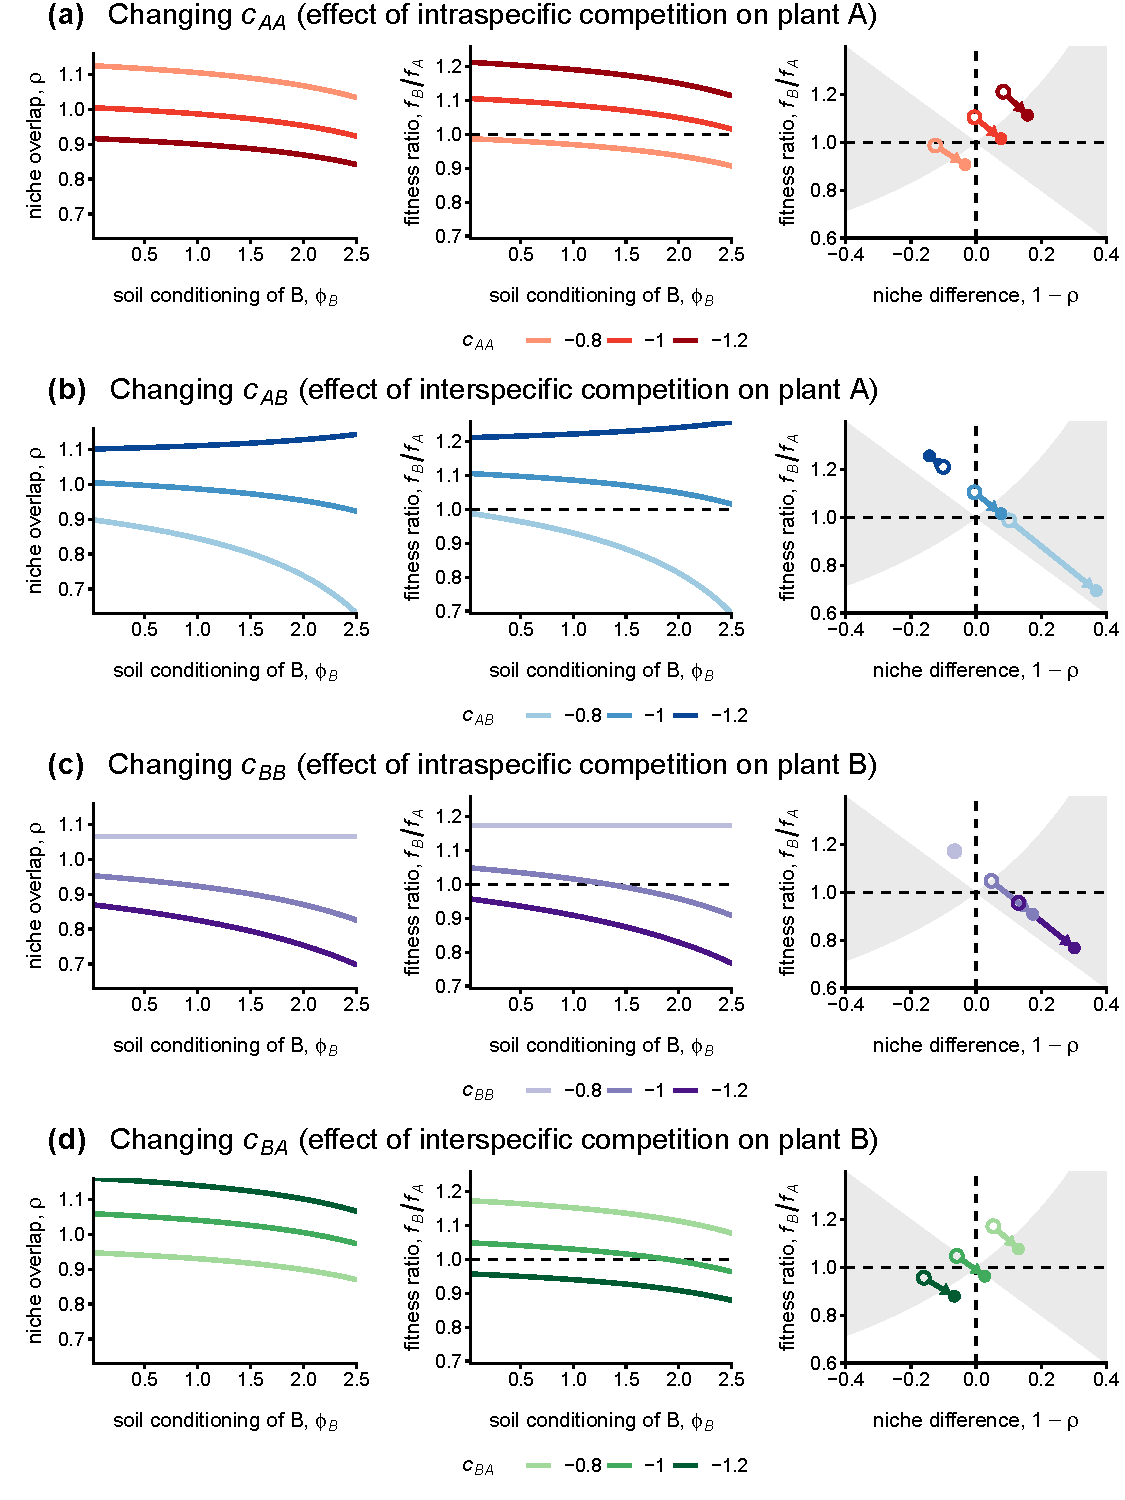
\includegraphics[width=12cm]{Chapter4/Translated_Soil_Conditioning_full.pdf}}
	\caption[The effects of varying plant--soil microbe interactions ($\phi_{B}$) and plant--plant competition on competition outcomes for the differential soil conditioning scenario.]
		{The effects of varying plant--soil microbe interactions ($\phi_{B}$) and plant--plant competition on competition outcomes for the differential soil conditioning scenario.
		Each row (panel a--d) represent the effects of varying one plant--plant competition coefficient while keeping the other three constant: (a) $c_{AA}$, in red colors; (b) $c_{AB}$, in blue colors; (c) $c_{BB}$, in purple colors; (d) $c_{BA}$, in green colors. Lines with different brightness represent different plant--plant competition strength, ranging from weak (light colors) to strong (dark colors).
		The first two columns represent the effects of varying $\phi_{B}$ on niche overlap ($\rho$) and fitness ratio ($f_{B}/f_{A}$), respectively. The third column visualizes the changes in the two components on the parameter space of niche difference ($1 - \rho$, x-axis) and fitness ratio ($f_{B}/f_{A}$, y-axis). Arrows represent the effects of changing plant--soil microbe interactions, from weakest (open circle) to strongest (solid circle). See also Fig.~\ref{fig:Scenario_Battleaxes} legend.}
	\label{fig:Soil_Conditioning_everything}
\end{figure}

